\chapter{Role of Tropospheric Jet Changes in the Interannual Variability and Decadal Trend of Asian Monsoon Rainfall}

\section{Abstract}
We have previously investigated the leading mode of July-August Asian monsoon variability (hereafter termed All-Asia EOF1) and argued that this mode manifests a coupling between the Himalayan Foothills and Yangtze River Valley. In this chapter, we investigate the manifestation of All-Asia EOF1 in JRA-55 reanalysis and associated atmospheric anomalies across the Northern Hemisphere. Extreme years of All-Asia EOF1 correspond to a global-scale Northern Hemisphere wavetrain known as the Circumglobal Teleconnection (CGT), leading to temperature and rainfall anomalies across the globe. Positive All-Asia EOF1 years are also correlated with a band of anomalous diabatic heating spanning the Himalayan foothills and Yangtze River valley also characterized by anomalous westerly moisture transport. Thus, JRA-55 reanalysis supports the hypothesis from Chapter 2 that changes in moisture transport across the Yunnan Plateau induce the All-Asia EOF1 pattern of rainfall response. In addition, we propose that East Asian heating can force the CGT, creating a trough and ridge pattern over central China and Siberia respectively that may contribute to the phase-locking of the CGT in summer, further strengthened by the effect of Asian high terrain.

Over East Asia, positive All-Asia EOF1 years feature a robust southward shift in the tropospheric jet, and vice-versa in negative years. We search for further links between the position of the East Asian jet and rainfall anomalies in the East Asian monsoon on an interannual and interdecadal time scale using the RDA catalog presented in Chapter 3. The frequency of banded rainfall during the Pre-Meiyu and the latitude of rainbands during the Post-Meiyu are both found to covary with meridional shifts of the tropospheric jet. Furthermore, major late-twentieth-century changes in the frequency and latitude of frontal rainfall (the ``South Flood-North Drought'') are found to coincide with anomalies in East Asian jet latitude. The East Asian jet has likely responded both to decadal changes in regional temperature and to \nth{20}-century global warming. Though the mid-latitudes force East Asian monsoon weather chaotically (the ``Silk Road'' pattern), idealized studies and high-resolution global climate models have begun to converge in their projections of future East Asian jet changes and the Circumglobal Teleconnection under \nth{21}-century warming. Given the observational relationship shown herein between the East Asian jet, CGT and anomalous rainfall, the potential exists to improve projections of twenty-first-century rainfall change in China, which remained highly uncertain in the latest International Panel on Climate Change report (IPCC5).

\section{Introduction}

	In many of the world's most populous regions, the duration and severity of monsoon rainfall dictates the well-being of the populace by controlling crop yields, flooding and freshwater supply. The history of monsoon study is therefore replete with attempts at its prediction dating back over a century, such as the India Meteorological Department (IMD)'s official seasonal forecast (available at \url{http://www.imd.gov.in/pages/monsoon_main.php}) and recent concerted efforts such as the `Seasonal Prediction of the Indian Monsoon' (SPIM) project \citep{Gadgil2011}. Nonetheless, IMD operational forecasts of the Indian monsoon demonstrated no skill over the years 1989-2012 \citep{Wang2015}. Past generations of global climate models have struggled even to produce a realistic mean state for the Indian monsoon \citep{Gadgil2003}, let alone its variability \citep{KrishnaKumar2005}. 
	
	An even bigger challenge awaits in the prediction of the future of the monsoon under global warming. Twenty-first-century changes in mean temperature and rainfall will impact the livelihood of billions \citep{Barrios2010,Burke2015}. Unfortunately, in the latest iteration of the Intergovernmental Panel on Climate Change report (IPCC5), it is acknowledged that models struggle to produce realistic patterns of rainfall in the Asian monsoon region due to the heterogeneity of high terrain \citep{Christensen2011}. Weak consensus exists between models on twenty-first-century rainfall increase in China under their RCP4.5 scenario, and only ``medium confidence'' in increasing rainfall during the South Asian summer monsoon. At a more fundamental level, even simplified (aquaplanet) versions of the CMIP5 models respond entirely differently under elementary climate perturbations such as a uniform 4K temperature increase, due primarily to their inability to parametrize moist convection and cloud formation in a physically realistic way \citep{Stevens2013}. Therefore, even in regions where the models do arrive at a consensus, it is not clear that their projections should be trusted. Meanwhile, from a theoretical standpoint, it is debated whether the future Asian monsoon could undergo nonlinear change under global warming \citep{Zickfeld2005}, or will instead evolve linearly \citep{Boos2016}.
	
	In this chapter, we focus on the leading mode of Asian monsoon rainfall variability, named All-Asia JA EOF1 in \citet{Day2015}, and its relation to other regional and global modes of climate variability. All-Asia JA EOF1 (hereafter referred to as All-Asia EOF1 for convenience) features enhanced precipitation over the Himalayan Foothills and Yangtze River corridor in its positive phase and decreased precipitation over the Monsoon Zone, northern China and southernmost China, and vice-versa in its negative phase. We first find using composite analysis that All-Asia EOF1 is correlated with a wavelike pattern of anomalies across the Northern Hemisphere known as the Circumglobal Teleconnection (CGT). In the second, we find that the South Flood-North Drought pattern of twentieth-century rainfall change in China was also accompanied by changes in the East Asian jet. Thus, All-Asia EOF1 rainfall variability implies a corresponding set of atmospheric changes at the scale of the entire Northern Hemisphere.
	
	The CGT and the East Asian tropospheric jet respond to global modes of climate variability and will be influenced by \nth{21}-century global warming. The CGT is defined as the second EOF of summer midlatitude geopotential height variability (EOF1 reflects ENSO). In the past several decades, severe heat waves and droughts have been ascribed to high-wavenumber standing Rossby wave circulations \citep{Schubert2011}. In several cases, Eurasian heat waves were directly tied to South Asian monsoon extremes \citep{Lau2012,Trenberth2012}. Current debate investigates whether polar amplification observed in \nth{20}-century warming will make midlatitude blocking events more frequent and severe \citep{Francis2012}, or not \citep{Barnes2013,Hassanzadeh2014a}. The response of the the tropospheric jet to climate change has also been extensively studied. The jets marks the poleward boundary of the Hadley Cells \citep{Bordoni2008}, and therefore shift in response to global changes in inter-hemispheric heating gradient\citep{Chiang2012}. Therefore, it can be argued that the jet translates global climate forcings into regional climate change. Observations show a poleward shift in previous decades in response to global warming \citep{Fu2006,Archer2008,Fu2011}, but the opposite trend is found over East Asia \citep{Yu2007, Archer2008,Park2014a}. The poleward expansion of the Hadley Cell is projected to continue under \nth{21}-century warming \citep{Frierson2007,Lu2007,Kang2012}, but a recent study predicts that anomalous \nth{21}-century heating of the eastern Pacific Ocean will continue to push the East Asian jet further equatorward \citep{Park2014}.
	
	In summary, much work has already been done to anticipate changes in the CGT and the tropospheric jet on a warmer planet. By showing in this chapter that both of these climate components and the All-Asia EOF1 mutually influence one another, we open the possibility of using projections of midlatitude blocking and shifting of the tropospheric jet on a warmer planet to inform projections of the \nth{21}-century Asian monsoon.

%% ADD ALL RELEVANT CITATIONS TO PARAGRAPHS BELOW
\section{Data and Methods}

\subsection{JRA-55 Reanalysis}

	We rely on the JRA-55 reanalysis product assembled by the Japanese Meterological Association (JMA) \citep{Kobayashi2015,Harada2016}. JRA-55 is a state-of-the-art 56-year (1958-2013) reanalysis product, the first since ERA-40 to cover the past half-century. The realism of model climate is notably improved from the previous generation product, JRA-25, due in part to a brand new assimilation scheme. Fields are calculated at a model resolution of up to 640 $\times$ 320 (.625$^{\circ} \times .625^{\circ}$), with exact number of longitude points varying by latitude. The products used in this analysis are upscaled to 1.25$^{\circ} \times 1.25^{\circ}$. Monthly fields at the 700-mb, 500-mb and 200-mb levels were used, as well as column-integrated values where applicable. We calculated monthly anomalies in JRA-55 fields for positive and negative composites of years (described below), and also calculated normalized anomalies by finding the monthly standard deviation of each field for each calendar month. For a field $X$ and calendar month $m$, we calculate the monthly standard deviation $\sigma_{X_m}$ as follows:
	
\begin{equation*}
	\sigma_{X_m}(x,y)=\left(\sum_{56\ years} \left(X_m(x,y,yr)-\overline{X_m(x,y)}\right)^2 \right)^{1/2}
\end{equation*}
	
\subsection{Historical Precipitation and Temperature Records}

	We rely on the University of Delaware precipitation data set (hereafter referred to as UDEL) v4.01, available at $.5^{\circ} \times .5^{\circ}$ resolution (land only) for the years 1900-2014 \citep{Matsuura2015}. Data are assimilated from station records before being interpolated onto the grid, with quality control algorithms applied to weed out faulty records. For the testing of statistical significance, we use the same years as available in JRA-55, 1958-2013, which also feature higher station coverage than the first half of the \nth{20} century.

	Monthly temperature anomalies from 1958 to 2013 gridded at $1^{\circ} \times 1^{\circ}$ resolution were obtained from the Berkeley Earth Surface Temperature project (hereafter referred to as BEST), freely available at \url{http://www.berkeleyearth.org/data/} \citep{Rohde2012}. BEST agrees closely with past historical temperature estimates, but the gridless methodology used can incorporate a wider range of temperature records \citep{Rohde2013}. According to their best estimate, global land mean temperature increased by $.89 \pm .06^{\circ}$C from 1950-1959 to 1990-1999. Therefore, in order to compare local temperature anomalies on an even footing, the temperature time series are detrended based on 1958-2013 local slope. At each point, we separate the time series into 12 separate monthly time series (each consisting of 56 Januarys, Februarys and so on) and then detrend each monthly time series based on the 56-point trend in that month.
	
\subsection{Composite Analysis}		
	
	We construct positive and negative composite anomalies for July and August from JRA-55 data, UDEL precipitation and BEST temperature. Positive composite years were chosen by selecting the five years between 1958 and 2007 when the value of All-Asia EOF1 was highest \citep{Day2015}. We then create a positive composite anomaly by averaging over fields in those five years and subtracting from the 56-year mean (1958-2013). The same procedure was repeated for the 5 most negative July All-Asia EOF1 years in the same timespan, and then the entire process repeated for the month of August. Further detail on selected years is included in Tables \ref{tab:t41}. Most figures in this paper show the \textit{difference} between the positive and negative composites, or ``inter-composite difference,'' except where otherwise stated.
	
	%again, can mention compositing with All-Nepal Monsoon Rainfall, but non-essential to chapter.
	
\subsection{Montecarlo Estimates of Statistical Significance}	
	
	Two methods are used to calculate the statistical significance of inter-composite differences: An analytic calculation based on the monthly standard deviation, and a Montecarlo method that generates arbitrary composites with 10,000 iterations. 

\subsubsection{Analytic Calculation}	
	
	The analytic method approximates the distribution of anomalies as Gaussian. For a field of interest $X$ in month $m$, we construct positive composite $X_{m+}$, negative composite $X_{m-}$ and normalized inter-composite difference $Z_{X_m}$ with total number of observation months $N$ and monthly standard deviation $\sigma_{X_m}$:
	
\begin{align*}
	X_{m+} &= \left(X_{m+,1}+X_{m+,2}+X_{m+,3}+X_{m+,4}+X_{m+,5}\right)/5 \\
	X_{m-} &= \left(X_{m-,1}+X_{m-,2}+X_{m-,3}+X_{m-,4}+X_{m-,5}\right)/5 \\
	Z_{X_m} &= \frac{N^{1/2}\left(X_{m+} - X_{m-}\right)}{\sigma_{X_m}}
\end{align*}

	$Z_{X_m}$ can then be converted to a $p$-value assuming that anomalies are normally distributed.

\subsubsection{Montecarlo Method}	
	
	For each iteration of the Montecarlo method, we create random non-overlapping positive and negative composites of five random years each from any of the 56 Julys (and analogously for August) and then find the inter-composite difference at each spatial point. At the end of 10,000 iterations, we find an effective $p$-value at each point by comparing the actual composite difference to the 10,000 simulated differences. The Montecarlo method is generally found to be a much stricter test of significance. Figures showing statistical significance use Montecarlo-estimated $p$-values. We also calculate an additional p-value for the entire pattern, namely the probability that the total \textit{area} exceeding a 95\% confidence level could be obtained at random. Since we are particularly interested in the Northern Hemisphere midlatitudes, we sum the total significant area between 20$^{\circ}$N and 65$^{\circ}$N and divide by total area. This ``pattern'' $p$-value is listed on the top-right of figures when calculated with region of interest marked on each figure. Since the test statistic in this case is one-sided, a pattern $p$-value exceeding .95 would be significant at a 95\% confidence level.

\subsection{Jet Count Density} 

	\citet{Schiemann2009} constructed a data set of jet ``counts'' in the Tibetan Plateau region (46$^{\circ}$ E-130$^{\circ}$ E, 17$^{\circ}$ N-58$^{\circ}$ N) from ERA-40 reanalysis for 1958-2001, where a count is defined as any local maximum in zonal wind with westerly magnitude greater than $30$ m s$^{-1}$; further details can be found in section 2 of \citet{Schiemann2009}. We show daily mean jet latitude averaged across $90^{\circ}-130^\circ$E in Figure~\ref{fig:jet_seasonal}a and monthly anomalies in Figure~\ref{fig:jet_seasonal}b and c. Results are not sensitive to the choice of longitude range. Figure~\ref{fig:climo} presents contours of jet frequency estimated by a kernel density method, which estimates a probability distribution from a set of discrete data observations. The \citet{Schiemann2009} database is also tested for covariance with the Rainband Detection Algorithm (RDA) catalog from Chapter 3 as shown in Figure~\ref{fig:jet_seasonal}, with results described subsequently.
	
\section{Composites of All-Asia EOF1 in JRA-55}

\subsection{Circumglobal Teleconnection}

	We build composites of the most positive and negative years of All-Asia EOF1 and find robust global change in upper-tropospheric height (Z200) across the Northern Hemisphere. The largest signal is a massive rise in geopotential height in the Tropics in the July composite, a known phenomenon in strong ENSO years (Figure~\ref{fig:cgt_zonal}), even though All-Asia EOF1 is not significantly correlated with ENSO. The absolute magnitude of anomalies in the Tropics remains less than in mid-latitudes because its variability is much lower (sidebar of Figure~\ref{fig:cgt_zonal}a). To focus on wavelike mid-latitude behavior, we subtract the zonal mean anomaly in subsequent figures where useful, as shown for instance in Figures~\ref{fig:cgt_zonal}c and~\ref{fig:cgt_zonal}d.
	
	In July (Figure~\ref{fig:cgt_z}a), strong All-Asia EOF1 years are associated with a zonal wavenumber 5 standing wave spanning the entire Northern Hemisphere. Analyzing 200-mb geopotential height (Z200),  pronounced positive lobes are visible over Russia, the eastern Pacific, western North America and the Azores, and negative lobes over Pakistan, northeast Asia and northern Europe. In August (Figure~\ref{fig:cgt_z}b), a similar pattern is obtained with some shifts: the northeast Asian lobe bifurcates into a Korean and Aleutian pair, the Siberian high strengthens and the North American high merges with that in the Eastern Pacific. Both the July and August Z200 anomaly patterns are significant at a 95\% confidence level. Considering the mid-troposphere and near-surface, we find that geopotential height anomalies are mostly barotropic and remain visible at the 700-mb level, except for over Pakistan where the 200-mb low is replaced by a surface high, and a belt from the eastern Tibetan Plateau eastward with 200-mb highs and 700-mb lows (Figure~\ref{fig:cgt_qq}a-b). These reflect cooling over Pakistan and heating over northern India, the Yangtze River Valley and western Pacific. All patterns are significant at a 95\% level except for Z700 in August.
	
	These patterns strongly resembles the Circumglobal Teleconnection (hereafter CGT) studied in \citet{Ding2005a}. \citet{Branstator2002} originally found that, in regions of strong meridional temperature gradient such as East Asia, a pattern with zonal wavenumber 5 can extend around the globe, with the tropospheric jet serving as a waveguide favoring the zonal propagation of storms. They were able both to find evidence of such a mode in reanalysis and demonstrate its existence in a simplified model. Figure 1c of \citet{Branstator2002} closely resembles our Figure~\ref{fig:cgt_zonal}d. Looking more closely at Figures 5b and c of \citet{Ding2005a} we find that they are practically identical to our Figures~\ref{fig:cgt_z}a and~\ref{fig:cgt_z}b (with sign inverted), including the set of changes between July and August. Furthermore, geopotential height anomalies of the studied global wavetrains in both \citet{Branstator2002} and \citet{Ding2005a} are consistently barotropic except over India (Figure~\ref{fig:cgt_z}). It should be noted that the CGT was also found to operate in June and September; for our purposes, we focus on its manifestation in July and August. We conclude that the mid-latitude wavetrain associated with All-Asia EOF1 and the CGT as defined by \citet{Ding2005a} are the same pattern.
	
	Another way of displaying the same wavetrain pattern is to consider the upper-level meridional wind (V200). Since the zonal mean of meridional wind is 0 and also near-zero in composites, waves are apparent without additional filtering \citep{Branstator2002}. Figure~\ref{fig:cgt_v} shows V200 for the July and August composites. The number of lobes can easily be counted, and the July wavetrain appears to be of wavenumber 6 while August is of wavenumber 5. From the Aleutian Islands to the eastern United States, the pattern of meridional wind anomalies in fact reverses from July to August, while remaining largely similar over Eurasia, showing substantial change between July and August. The existence of substantial differences between the July and August wavetrain patterns was also found in \citet{Ding2005a}. Although \citet{Day2015} argues that July and August All-Asia EOF1 are highly similar over the Asian monsoon region, this is evidently not true at the global scale.
	
	Finally, we consider the global distribution of temperature and precipitation anomalies associated with All-Asia EOF1 (Figure~\ref{fig:cgt_pt}). Positive and negative temperature composites were derived from detrended monthly temperature anomalies from BEST, while precipitation composites were obtained from University of Delaware's monthly precipitation record, as described in greater detail in the Methods section. In general, surface temperature increases are inversely correlated with precipitation, presumably because more energy is stored as latent heat in wetter years. Only a few regions outside of South and East Asia show significant anomalies. Most robustly, the Pamir and Tianshan Mountain region, including Tajikistan, Kyrgyzstan and the Taklamakan Desert of western China, moisten and become colder in positive All-Asia EOF1 years. This can be seen in the original figure showing All-Asia EOF1 in \citet{Day2015}, and is likely associated with changes in the tropospheric jet shown in Figure~\ref{fig:cgt_u}. Robust warming is found over almost all of India, the Arabian Peninsula and the eastern Sahara in positive years, and also to the north over central Siberia, which is the site of a strong atmospheric ridge visible in Figure~\ref{fig:cgt_z}. Patterns are generally quite similar to Figures 7 and 9 in \citet{Ding2005a}, although ours feature lower amplitude outside of the Asian monsoon.
	
	Recent work finds an associated between high-wavenumber Northern Hemisphere summer standing wave patterns and extreme climate events such as Eurasian heat waves that may have been aggravated in recent decades by global warming \citep{Petoukhov2013,Schubert2014a}. The July composite shows strong warming over Russia, cooling over the United Kingdom, northwestern Europe and southern Scandinavia, and rainfall increase over Scandinavia (Figure~\ref{fig:cgt_pt}a). However, the general sparsity of significant anomalies and differences between July and August suggest that the phase of All-Asia EOF1 does not translate to a consistent pattern of temperature and precipitation anomalies across Eurasia.
	
%%% PARAGRAPH ON PREDICTIVITY OF ALL-NEPAL MONSOON RAINFALL - probably not strong enough to be included, unnecessary.	
%	In \citep{Day2015}, we discussed the potential of All-Nepal Monsoon Rainfall (ANMR) as representative of All-Asia EOF1-type variability. Here we show that ANMR has some predictive power on CGT-type patterns. Using a different set of composite years chosen as extreme years of All-Nepal Monsoon Rainfall (Table~\ref{tab:t42}), we repeat the process in Figure~\ref{fig:cgt_z} for July (several years overlap with peak All-Asia EOF1 years). In August, only a faint CGT pattern is found (not shown), so it may be more reasonable to suggest that the CGT and All-Nepal Monsoon Rainfall are both driven by the same external variability.  

\subsection{Regional Changes Associated with All-Asia EOF1}

\subsubsection{Moisture Transport Across the Yunnan Plateau}

	We examine the regional dynamics within the Asian monsoon that potentially drive All-Asia EOF1-type variability. Furthermore, we can test the hypothesis in \citet{Day2015} that changes in moisture transport across the Yunnan Plateau couple the Himalayan Foothills and Yangtze River Valley and drive All-Asia EOF1. JRA-55 surpasses its predecessors in model resolution and may therefore provide a more credible picture of Asian monsoon dynamics.
	
	%%may also be the case that the model was specifically designed to perform well with Asian monsoon.

	We consider the distribution of diabatic heating within the South and East Asian monsoons associated with All-Asia EOF1. The column-integrated heating $Q$ is calculated according to JRA-55 as the residual of the sum of total column upwelling and downwelling short-wave fluxes $\Delta R_S\uparrow$ and $\Delta R_S\downarrow$, upwelling and downwelling long-wave radiative fluxes $\Delta R_L\uparrow$ and $\Delta R_L\downarrow$, sensible heat flux from the surface  $\Delta SH_{sfc}$ and latent heat flux  $\Delta LH=L \dot P$, all provided as monthly products in JRA-55:
	
\begin{equation}
	Q=R_{S_{top}\downarrow}-R_{S_{sfc}\downarrow}-R_{L_{sfc}\downarrow}-R_{S_{top}\uparrow}+R_{S_{sfc}\uparrow}-R_{L_{top}\uparrow}+R_{L_{sfc}\uparrow}+SH_{sfc}\uparrow+LP
\end{equation}
	
	$L$ is the latent heat of condensation of water vapor and $P$ precipitation. With our composite analysis, we find massive $Q$ fluxes in the Asian monsoon region associated with our pattern (Figure~\ref{fig:cgt_qq}). The radiative equilibrium is dominated by latent heat flux, which is an order of magnitude larger than the other terms (their magnitude generally maximizes at 10 W m$^{-2}$). Significantly, there are no other regions of concentrated Q-fluxes, which suggests that the Asian monsoon region is forcing the CGT in these years.
	
	%WAVE ACTIVITY FLUX COULD HELP PROVE THIS
	
	Figure~\ref{fig:cgt_dyn} focuses on the Asian monsoon region (10$^{\circ}$E-170$^{\circ}$W and 5$^{\circ}$N-50$^{\circ}$N) and only show composite differences that are statistically significant. In both July and August, the Himalayan Foothills and the Yangtze River Valley are a site of diabatic heating, with cooling observed over the Monsoon Zone of India, the Bay of Bengal and the South China Sea (Panels a and b). Almost all anomalies in $Q$ are again driven by anomalous latent heat fluxes. The positive heating anomaly corresponds to a coherent belt of surplus water vapor and anomalous ascent stretching from the Himalayan Foothills and the southeastern Tibetan Plateau eastward to the Yangtze River Valley, and onward to South Korea and Japan (Panels c-e). This same belt is also characterized by low- and mid-level westerly wind anomalies and enhanced eastward moisture transport. The general spatial distribution of anomalies closely matches All-Asia EOF1 in \citet{Day2015}. We suggest that changes in the transport of water vapor from the Bay of Bengal supply additional energy as latent heat and drive patterns of diabatic heating. 
	
	To substantiate this claim, we separately examine column-integrated moisture transport in each of the positive and negative composites (not shown). In positive composite years, the magnitude of southward water vapor transport northward in southern China reaches 250 kg m$^{-1}$ s$^{-1}$ versus only about 170 kg m$^{-1}$ s$^{-1}$ in negative years. In addition, the eastward moisture transport in positive composite years across the Yunnan Plateau is roughly 100 kg m$^{-1}$ s$^{-1}$, and near-zero in negative composite years (in fact, low-level winds are slightly easterly across the Yunnan Plateau in August per JRA-55). Therefore, JRA-55 suggests that Bay of Bengal moisture is a major summer source of moisture for the East Asian monsoon, and also highly variable. The magnitude of flux from the Bay of Bengal almost certainly does not contribute all of the latent heat flux anomaly, but may instead serve as a convective trigger leading to further diabatic reinforcement \citep{Sampe2010}.
	
	We also look separately at the positive and negative composites for further information on monsoon changes associated with All-Asia EOF1 (Figures~\ref{fig:cgt_700} and~\ref{fig:cgt_500}). In positive All-Asia EOF1 years, a tongue of air with high specific humidity stretches eastward from the Yunnan Plateau into the western Pacific (Figure~\ref{fig:cgt_700}a). We can also see that low-level convergence and mid-tropospheric ascent are anchored at 30$^{\circ}$N. In negative All-Asia EOF1 years monsoonal flow penetrates much further north, reaching about 35$^{\circ}$N, northern China becomes more convectively favorable between 35$^{\circ}$N and 40$^{\circ}$N and the Yangtze River Valley features only weak ascent. Figure~\ref{fig:cgt_500} also appears to show southwest-northeast shifts of the West Pacific subtropical high, reminiscent of Pacific-Japan pattern variability \citep{Kosaka2011}
	
	Other notable changes occur elsewhere in the Asian monsoon region. The Monsoon Zone of central India features a local maximum in specific humidity in negative All-Asia EOF1 years (Figure~\ref{fig:cgt_700}b, about 10 g kg$^{-1}$) that is absent in positive years. Arid northwestern India is a location of high All-Asia EOF1 amplitude, which can be understood by considering Figures~\ref{fig:cgt_700} and~\ref{fig:cgt_500}. In positive All-Asia EOF1 years the northwesterly winds bring hot, extremely dry air from Pakistan to northwestern India, whereas in negative years the region receives a southeasterly source from the Bay of Bengal across the Monsoon Zone. The Arabian Sea is never a source of moisture to northwestern India in spite of its proximity. Northwestern India also varies between near-zero vertical pressure velocity and being convectively favorable in positive and negative years respectively. Finally, in negative All-Asia EOF1 years, the southern Bay of Bengal and parts of southeast Asia become much more favorable to ascent, as well as the windward side of low mountain ranges such as the Ghats and the Philippines coastal range (Figure~\ref{fig:cgt_500}). All of the changes described in this paragraph are statistically significant according to Figure~\ref{fig:cgt_dyn}.
	
\subsubsection{Meridional Shift of the East Asian Jet}

	Over East Asia, Figures~\ref{fig:cgt_u}a and b reveal that positive All-Asia EOF1 Julys and Augusts are both marked by a \textit{robust southward shift of the jet} between 50$^{\circ}$E-150$^{\circ}$E, with significance of hemispheric change exceeding a 99\% level. We independently examine jet position in the positive and negative composites for each of July and August (Figures~\ref{fig:cgt_u}c-f). In the Asian monsoon region, the climatological position of the jet (with core roughly marked by 30 m s$^{-1}$ and 36 m s$^{-1}$ in Figures~\ref{fig:cgt_u}c-f) is strongly influenced by underlying high topography. We expect high orographic barriers such as the Tibetan Plateau to force deviations in overlying circulation by conservation of potential vorticity, wherein the rotation of the earth encourages atmospheric circulation to move as sets of uniform incompressible columns \citep{Holton2004a}.
	
	The high terrain of the Iranian Plateau upstream from the Tibetan Plateau induces a climatological northward meander in the jet. In positive All-Asia EOF1 years the amplitude of this deviation is small, and the jet returns southward before interacting with the Tibetan Plateau and being forced northward again, with northern apex and maximum velocity over the Taklamakan Desert. The jet then returns southward of 40$^{\circ}$N at the longitude of Eastern China. A strong core beginning around South Korea and Japan persists well into the Northern Pacific, past the International Date Line. In negative All-Asia EOF1 years (Panel e), the northward meander around the Iranian Plateau is particularly large, and accompanied by a strong maximum velocity in the vicinity of Kazakhstan and Uzbekistan in excess of 40 m s$^{-1}$. The jet returns southward over the Tianshan Mountains, but then recurves northward across northeastern China, North Korea and Vladivostok. At some longitudes such as 70$^{\circ}$E and 130$^{\circ}$E the difference in latitude exceeds 5$^{\circ}$ (over 500 km).
	
	In summary, the CGT corresponds to a meridional jet shift over East Asia. This shift appears zonally uniform, but a closer inspection reveals that the climatological position of the jet is strongly constrained by regional high topography in both positive and negative All-Asia EOF1 years.
	
\subsection{East Asian forcing of the CGT}

	The forcing of the Circumglobal Teleconnection has been debated in the literature. \citet{Ding2005a} found that the Indian summer monsoon was a major driver of the CGT, while ENSO influence was not significant except through indirect forcing of the Indian summer monsoon. They also found that the North Atlantic jet exit (50$^{\circ}$E), a region of high variability in geopotential height and baroclinic instability, can stimulate the CGT by conversion of mean state flow to kinetic energy. \citet{Ding2007} further investigated the time-lagged propagation of midlatitude disturbances from the North Atlantic and found that they can trigger active and break spells in the Indian monsoon (analogous to negative and positive All-Asia EOF1 respectively), although the actual mechanism of triggering remains unclear. In their view, the diabatic heating from the Indian monsoon strengthens the Central Asian high and a Siberian high that brings anomalous rainfall to North China.
		
	We propose a third component of CGT forcing in addition to the Indian monsoon and North Atlantic: Diabatic heating from the Himalayan Foothills and Yangtze River Valley. In positive All-Asia EOF1 years, widespread cooling over India, the Indian Ocean and southeast Asia predominates, but a coherent band of heating from 90$^{\circ}$E to 130$^{\circ}$E exists of order 100 W m$^{-2}$. As previously argued above, this heating results from increased moisture transport from the Bay of Bengal eastward across the Yunnan Plateau to central China, triggering a diabatic feedback and heating from increased latent heat flux. While the area of cooling in India and southeast Asia exceeds the total heating along this pathway, Yangtze River Valley heating predominates in East Asia and appears as a major source on the global level (Figure~\ref{fig:cgt_qq}). Central China heating may also induce the phenomenon of ``phase-locking'' in the CGT, wherein the standing wave has preferred configurations. It is known that the winter analog of the CGT has no preferred phase \citep{Branstator2002} but its summer component does \citep{Ding2005a}. We propose that the surplus summer diabatic heating over central China in positive All-Asia EOF1 years creates a trough-and-ridge configuration over the Yangtze River Valley and Siberia to its northwest, which anchors the position of the CGT wavetrain over East Asia. This phase-locking is reinforced by the strong interaction of the East Asian jet with surface topography seen in Figure~\ref{fig:cgt_u} which restricts the East Asian jet to particular configurations. Therefore, we propose that \textbf{the geometry of the Tibetan Plateau and Yunnan Plateau lead to the summer phase-locking of the CGT, firstly by steering moisture transport from the Himalayan Foothills to the Yangtze River Valley and inducing diabatic heating, and secondly by topographic deflection of the East Asian jet}.

%Inez had good way of summarizing Meiyu changes: 1) timing 2) frequency 3) intensity.
\section{East Asian Jet Shifts and the South Flood-North Drought}

\subsection{Overview}

	In the previous section, we showed that positive and negative All-Asia EOF1 years are reflected as zonally coherent southward and northward shifts of the East Asian Jet extending into the northwestern Pacific Ocean. This relation of East Asian jet latitude and rainfall in July and August leads us to investigate a link between jet position and China rainfall in other seasons using the Rainband Detection Algorithm (RDA) catalog established in Chapter 3. 
	
	It is well known that the jet plays a crucial role in the climatology of the Asian monsoon and the transport of storms to East Asia. The onset of the South Asian monsoon corresponds to the passage of the tropospheric jet north of the Tibetan Plateau \citep{Yin1949,Yeh1959,Hahn1975}. The interaction of the jet and Tibetan Plateau produces a standing wave that encourages convergence and ascent downstream over China and the Western Pacific during Meiyu Season \citep{Yang2002,Molnar2010,Chen2014}. The jet also serves as a waveguide for storms propagating from the Eurasian interior via the ``Silk Road'' teleconnection \citep{Kosaka2012}, a regional manifestation of the Circumglobal Teleconnection \citep{Hoskins1993,Ambrizzi1997,Park1997}. There is also evidence connecting shifts in the East Asian jet with anomalous rainfall over China on an interannual time scale \citep{Liang1998,Du2009,Li2014}, and with the South Flood-North Drought pattern of decadal change in China \citep{Yu2004,Yu2007,Xuan2011}. 
	
	It has previously been argued that decadal change in the East Asian jet is strictly a local response to altered heating in the East Asian monsoon \citep{Yu2007}. However, the tropospheric jet shifts with meridional shifts of the Hadley Cell \citep{Kang2011a}, which are in turn forced by changes in interhemispheric heating gradient \citep{Chiang2012,Donohoe2013,Schneider2014}. Therefore, it is reasonable to suggest that the East Asian jet may have respond to twentieth-century external climate forcing on a global scale and translate it into regional impact. We do not suggest that the jet does not exclusively control the position of rainbands in China, but rather that a mutual feedback may exist between jet position and Meiyu rainfall. Such a feedback might also help with improving projections of changes in the twenty-first-century East Asian monsoon.
	
	Previously in Chapter 3, we used the RDA catalog to break the South Flood-North Drought down into changes in frequency, latitude and intensity during particular Meiyu stages. The most important contributors to decadal change were a decline in the frequency of fronts in May (the Pre-Meiyu), and a southward shift in rainband latitude during July-August (the Post-Meiyu). We now test whether decadal jet changes have also occurred during these stages, and more generally whether interannual changes in rainfall properties and changes in jet position are correlated.
	
\subsection{Climatology of the East Asian Jet}

	The East Asian jet assumes a different configuration during each of the five rainfall stages of East Asian monsoon rainfall described in Chapter 3. A full monthly jet climatology is presented in \citet{Schiemann2009}. Beginning in May, the East Asian jet moves from its winter position on the southern flank of the Tibetan Plateau to a summer latitude well north of the plateau. During this transition, the jet occupies intermediate configurations that correspond to different stages of China rainfall (Figure~\ref{fig:climo}). Peak rainfall rates in China from May to mid-July corresponds to the months when the climatological latitude of the jet impinges on the Tibetan Plateau, because the interaction of the tropospheric jet and Tibetan Plateau strengthens convergence and rainfall downstream over China and the western Pacific Ocean \citep{Molnar2010,Sampe2010,Chen2014}. From May to September,  the climatological latitude of rainfall, rainbands and jet density are all closely coupled, with peak jet density occurring 5 to 10 degrees north of the latitude of peak rainfall, as is expected in theory in a region of strong fronts \citep{Holton2004}. 
	
	Focusing on individual stages, we can see that the Pre-Meiyu period corresponds to the beginning of the jet's northward transit from its winter configuration. During Meiyu season, the preferred latitude of the jet continues to shift northward. The period of frequent double rainband occurrence during the Post-Meiyu occurs during the jet's maximal northward extent. Finally, the jet returns southward during the Fall Rains in October and November, which produces only a weak rainfall response. Thus, the East Asian monsoon is marked by a seasonal asymmetry between the jet's northward and southward passage, the former featuring strong rainfall and the latter much weaker amounts. Figures~\ref{fig:climo}a-e show mean rainfall, jet frequency and rainband position during each stage, as well as their zonal average (sidebars). From the Pre-Meiyu to Post-Meiyu, each northward jump in peak rainband frequency corresponds to a similar shift in jet count density.
	
\subsection{Jet Changes, 1980-2001 Versus 1958-1979}

	In Figure~\ref{fig:jet_seasonal}a, we show the zonal average over $90-130^\circ$E) of mean jet latitude, averaged over the years 1958-1979 (blue solid line) and 1980-2001 (dashed red line) with 95\% confidence intervals overlain. In Chapter 3, we found that changes in rainband properties were concentrated during the pre-Meiyu (May) and post-Meiyu (July-August). Changes in the jet are found during both of these time periods. During the Pre-Meiyu (May), the tropospheric jet is shifted southward by almost 2$^{\circ}$ in 1980-2001 relative to 1958-1979, when its mean latitude was $\approx 41^{\circ}$N. We estimate the significance of this change using a two-tailed Kolmogorov-Smirnov (K-S) test. Since the K-S test requires that all samples are independent, we first remove temporal autocorrelation due to synoptic variability by assimilating daily mean jet latitude into 4 day blocks (Figure~\ref{jet_autocorr}. A subsequent K-S test finds that the shift is significant at a 99\% confidence level with $p=0.003998$. During the Post-Meiyu (days 201-273), when a southward shift in rainband latitude is found in 1980-2001 relative to 1958-1979, the mean latitude of the jet is also consistently displaced southward. We assimilate daily mean jet latitude into 7-day blocks before performing a K-S test, and find a $p$-value of this shift of $p=0.05667$, which is not statistically significant.
	
	Figure~\ref{fig:changes_2d} overlays changes in jet kernel density over observed rainfall changes from APHRODITE during the Pre-Meiyu and the Post-Meiyu. Rainfall changes shown are for 1980-2001 versus 1958-1979 to match the length of the Schiemann database. Significant regions of yearly rainfall change are concentrated around 30$^{\circ}$N (increase) and 37$^{\circ}$N, mostly agreeing with Figure~\ref{fig:f31}. During the Pre-Meiyu (Panel b), the principal change is a decrease in jet counts around 30$^{\circ}$N, where rainfall and rainband frequency have also decreased significantly. During the Post-Meiyu (Panel c), we observe increased rainband probability around 28$^{\circ}$N and decreased rainfall and rainband frequency around 36$^{\circ}$N. Jet kernel density changes follow the same southward shift but with a 5$^{\circ}$ offset northward. The Post-Meiyu changes show a coherent set of changes in rainband, rainfall and jet position, while the Pre-Meiyu jet changes are more difficult to interpret directly.
	
\section{Hypothesis}

	A significant southward shift in the East Asian jet occurred during the Pre-Meiyu season between 1958-1979 and 1980-2001, as well as a weaker southward shift during the Post-Meiyu that was not statistically significant. In Chapter 3, we previously found a significant decrease in rainband frequency during the Pre-Meiyu, and a southward shift in rainband latitude during the Post-Meiyu. Here we suggest that both of these phenomena may have been caused by a southward shift in the seasonal cycle of the East Asian jet. Climatologically, rainfall surges during the Pre-Meiyu, which is also when the jet begins its northward transit and first impinges on the Tibetan Plateau. We propose that the date when the jet starts shifting northward has occurred later, thereby delaying the onset of the Pre-Meiyu and leading to a decrease in rainbands and rainfall. Subsequently, because the jet's northward progression has started later, its maximal poleward latitude is also further south, therefore decreasing rainfall in northern China and increasing rainfall in central China, and producing a South Flood-North Drought response. A similar argument was presented in \citet{Chiang2015} (the ``Jet Transition Hypothesis'') as a template for the effect of orbital forcing on the East Asian paleomonsoon.
	
	To test our hypothesis, we investigate the correlation of interannual anomalies in jet latitude to those of rainband properties during the Pre-Meiyu and Post-Meiyu. If interannual anomalies in jet latitude manifest as Pre-Meiyu changes in rainband frequency or Post-Meiyu changes in rainband latitude, our argument about the effect of interdecadal change in the East Asian jet becomes more plausible. Figure~\ref{fig:jet_seasonal}b shows a scatter plot of rainband \textit{frequency} anomalies versus jet latitude anomalies in May (days 121-150). Most years with a decrease in rainband frequency feature a southward jet shift, and vice-versa, and such years occur mostly during 1980-2007. A similar relation is found between monthly anomalies in rainband \textit{latitude} and jet latitude during July-August (days 201-260, Figure~\ref{fig:jet_seasonal}c). In the latter figure, we exclude rainbands south of 28$^{\circ}$N from calculated anomalies, since such rainbands reflect South China Sea storms, rather than jet influence \citep{Day2015}. Together, Figures~\ref{fig:jet_seasonal}b and~\ref{fig:jet_seasonal}c suggest that interannual changes in jet latitude affect Pre-Meiyu rainband frequency and Post-Meiyu rainband latitude.
	
	%%previously calculated statistical significance of these changes - should include!
	
	In summary, we propose that the delayed passage of the jet to the north of the Tibetan Plateau has delayed the onset of the Pre-Meiyu season, which has decreased May rainfall in central China, and restricted the northward advance of precipitation, thereby reducing Post-Meiyu rainfall in northern China. 	
		 
\section{Conclusion}

	The existence of a Circumglobal Teleconnection in Northern Hemisphere summer was demonstrated in models and observation in the past decade and a half. Two potential drivers of the CGT have previously been proposed: The Indian monsoon, where anomalies are baroclinic rather than barotropic and massive diabatic heating occurs, and baroclinicity in the Atlantic jet exit region, where geopotential height variability is particularly high. We propose a third source of CGT variability: Diabatic heating along the Himalayan Foothills and Yangtze River Valley of up to 100 Wm$^{-2}$ which produces a diagonally tilted trough-ridge pattern over China and Siberia. This characteristic dipole of geopotential height anomalies may encourage the phase-locking of the CGT in summer, further strengthened by the deflection of the jet by high topography across the Asian monsoon region. The magnitude of East Asian forcing does not necessarily overshadow the influence of the Indian monsoon and North Atlantic, but rather may complement it in strong All-Asia EOF1 years.
	
	We have shown that a significant amount of the annual and decadal variability in Meiyu front activity is accompanied by changes in the westerly jet. Both the Pre-Meiyu (May) and Post-Meiyu (July-August) seasons, during which the largest rainfall and rainband changes have occurred, feature a southward anomaly in mean jet latitude during 1980-2007 relative to 1951-1979. We argue that the previously discovered decline in Pre-Meiyu rainband frequency and southward shift in rainbands during the Post-Meiyu are both caused by an overall southward shift of the summer progression of the East Asian tropospheric jet, delaying Pre-Meiyu onset and restricting the northward range of banded rainfall. This interpretation is a modern analog of the Jet Transition Hypothesis described in \citet{Chiang2015}, wherein East Asian rainfall changes on paleoclimate timescales are ascribed to modulation in the seasonal cycle of the tropospheric jet. 	
	
	Composite analysis with JRA-55 also supports our chief hypothesis in Chapter 2, that changes in moisture transport across the southeastern Tibetan Plateau and Yunnan Plateau drive All-Asia EOF1 rainfall variability. According to our composite analysis, the source of Yangtze River moisture in July-August can vary from receiving a sizable Bay of Bengal component (up to 100 kg m$^{-1}$ s$^{-1}$) to being entirely sourced from the South China Sea. This claim can likely be tested with present-day records of precipitation isotopes. Since the transport distance from the Bay of Bengal to the Yangtze River is long, we would expect water arriving in central China from the west to be highly depleted, and therefore that positive All-Asia EOF1 years should see negative excursions in Yangtze River $\delta ^{18}$O records. This is also a region where many speleothems are located, cave stalagmites featuring tends of thousands of years of continuous deposition from which a continuous time series of $\delta ^{18}$O can be extracted. Traditionally, speleothem $\delta ^{18}$O records are viewed as proxies of local monsoon intensity. However, recent work increasingly argues that East Asian speleothem records such as Hulu and Sanbao are primarily a record of changes in the Indian monsoon upstream that are then transported downwind \citep{Pausata2011,Cai2015,Baker2015}. Proving that changes in water vapor transport from the Bay of Bengal alter the \textit{present-day} isotopic signature in central China would strengthen the new school of interpretation of East Asian speleothems.

	 In this chapter, we have shown a robust connection between Asian monsoon rainfall variability and two components of Northern Hemisphere summer climate, the Circumglobal Teleconnection and the tropospheric jet. In the case of the jet, we have shown that both interannual and decadal fluctuations in late-twentieth-century East Asian rainfall were also marked by a jet signal. The ultimate cause of the South Flood-North Drought remains unclear. Authors have suggested changes in Indian Ocean SST \citep{Qu2012}, decreased sensible heating from the Tibetan Plateau \citep{Liu2012a,Hu2015} and aerosol forcing \citep{Song2014}. We do not discuss the origin of the forcing here, but rather show that late-twentieth century change is consistently manifested across different climate elements. In particular, we open the possibility of using predictions about the tropospheric jet and the CGT under twenty-first-century global warming to improve projections of the future Asian monsoon. It is important to note that midlatitude forcing via the Silk Road teleconnection is intrinsically chaotic \citep{Kosaka2012}. Nonetheless, \citet{Lee2014} analyzed \nth{21}-century changes in a suite of CMIP5 models and concluded that the robust stabilization of the atmosphere in almost all models would tend to decrease the variability associated with the CGT. 
	 
	 For the tropospheric jet, observations show that the global annual mean latitude of the tropospheric jet has shifted poleward in tandem with the expansion of the Hadley circulation under global warming \citep{Fu2006,Archer2008,Fu2011}, and will continue to do so in future \citep{Lu2007,Kang2012}. However, the East Asian portion of the jet has shifted equatorward as found in our study and others \citep{Yu2007, Archer2008,Park2014a}, and recent work proposes that the southward trend will continue \citep{Park2014}. \citet{Liu2012} has already shown that transient forcing from the North Atlantic may have induced a response in the East Asian monsoon by shifting the pattern of westerlies. Based on the observed strong connections between the Circumglobal Teleconnection, East Asian Jet and Asian monsoon rainfall, we hope to use our growing knowledge of future behavior of other atmospheric components to improve the skill of projections of the twenty-first-century East Asian monsoon.

\section{Acknowledgments}

	Significant portions of the current work were produced in collaboration with Jacob Edman and John Chiang and under the guidance of Inez Fung. Computer code was written in MATLAB and Ferret. The formula for column-integrated heating was retrieved from the JRA-55 climatological atlas at \url{http://ds.data.jma.go.jp/gmd/jra/atlas/en/D_HEATcol.html}. University of Delaware precipitation is freely downloadable at \url{http://climate.geog.udel.edu/~climate/html_pages/download.html}. The UCAR Climate Data guide was used on several occasions to help select appropriate data products.

\newpage
\section{Tables and Figures}

%%%% TABLES %%%%

%% TABLE 4.1 - LIST OF YEARS USED IN POSITIVE AND NEGATIVE COMPOSITES OF ALL-ASIA EOF1	
\begin{table}[h]

\caption{Years used for the positive and negative composities of All-Asia EOF1 in July (July AA+ and AA-) and August (August AA+ and August AA-), expressed in units of standard deviation. Years are chosen as the most extreme values of All-Asia EOF1 as previously published in \citet{Day2015}.}
\centering
\begin{tabular}{ c c c c}
	 	 		\multicolumn{2}{c}{All-Asia EOF1 Composites} 	&			Years				&		Value (Std. Devs.)			\tabularnewline	
				\hline
	 \multirow{2}{*}{July} 		&  +							&	1970, 1987, 1998, 2002, 2007 	&	1.65, 2.25, 1.47, 1.35, 1.62		\tabularnewline
	 						&  -							&	1959, 1973, 1976, 1978, 1994       &	-1.59, -1.25, -1.45, -1.40, -2.65	\tabularnewline
	 \multirow{2}{*}{August}	&  + 							&	1958, 1965, 1993, 1998, 2005	&	1.85, 1.77, 2.00, 2.67, 1.49		\tabularnewline
	 						&  -  							&	1973, 1978, 1984, 1994, 2006	&	-1.96, -2.04, -1.68, -1.64, -1.40 	\tabularnewline

\end{tabular}
\label{tab:t41}
\end{table}

%%% TABLE 4.2 - LIST OF YEARS USED IN POSITIVE AND NEGATIVE COMPOSITES OF ALL-NEPAL MONSOON RAINFALL	
%\begin{table}[p]
%
%\caption{Years used for the positive and negative composities of July All-Nepal Monsoon Rainfall (July N+ and N-) and August All-Nepal Monsoon Rainfall (August N+ and August N-) expressed in units of cumulative rainfall (also translated into standard deviation. Years are chosen as the most extreme values of ANMR between 1961-2007, during which APHRODITE features high-quality station coverage \citep{Day2015}.}
%\centering
%
%\begin{tabular}{ c c c c}
%	 	 		\multicolumn{2}{c}{Nepal Composites} 	&			Years				&			Monthly Rainfall (mm)		\tabularnewline	
%				\hline
%	 \multirow{2}{*}{July} 		&  +						&	1984, 1985, 1988, 1998, 2007 	&	14.45, 13.45, 14.52, 13.51, 13.67		\tabularnewline
%	 						&  -						&	1971, 1973, 1991, 1993, 2006       &	9.04, 8.23, 8.12, 9.17, 9.16 			\tabularnewline
%	 \multirow{2}{*}{August}	&  + 						&	1961, 1962, 1966, 1988, 1998	&	12.47, 13.45, 11.88, 12.38, 13.83		\tabularnewline
%	 						&  -  						&	1972, 1984, 1986, 2004, 2006	&	6.62, 7.32, 7.82, 7.41, 7.78			\tabularnewline
%
%\end{tabular}
%\label{tab:t41}
%\end{table}
%
%\newpage
%\clearpage

\clearpage

%%%% FIGURES %%%%

%% FIGURE 4.1 - Composite geopotential height anomalies with and without zonal mean
\begin{figure}
\centering
\noindent\includegraphics[width=42pc]{Figures/ch4/CGT_zonal}
\caption{a) July composite difference in 200-mb level geopotential height (Z200) between positive and negative All-Asia EOF1 years. Sidebar: Zonal mean of composite anomaly. b) July Z200 composite anomaly expressed as Z-score (units of local std. devs.), showing massive anomaly in the Tropics. c) July Z200 composite anomaly with zonal mean removed, highlighting mid-latitude wavetrain. d) Same as Panel c, but expressed as Z-score as in panel b.}
\label{fig:cgt_zonal}
\end{figure}

%% FIGURE 4.2 - Geopotential height anomalies in upper troposphere, middle troposphere and lower troposphere (200mb, 500mb and 700mb)
\begin{figure}
\centering
\noindent\includegraphics[width=42pc]{Figures/ch4/CGT_z}
\caption{July All-Asia EOF1 composite difference in a) Z200, c) Z500 and e) Z700. Panels b, d and f are analogous to panels a, c and e except with procedure repeated for August. Local statistically significant differences at a 95\% level are marked by stippling. $p$-values at the top-right of each plot show the likelihood via Montecarlo testing that the \textit{amount of statistically significant area} between 20$^{\circ}$N and 65$^{\circ}$N (delimited on figures) could be achieved at random (given by $1-p$). A value above .95 indicates statistical significance at a 95\% confidence level.}
\label{fig:cgt_z}
\end{figure}

%% FIGURE 4.3 - July composite 200-mb meridional wind (V200 anomalies)
\begin{figure}
\centering
\noindent\includegraphics[width=36pc]{Figures/ch4/CGT_v}
\caption{Composite anomalies in 200-mb meridional wind (V200) in a) July and b) August, both of which show a robust global mid-latitude standing wave. As explained in Figure~\ref{fig:cgt_z} and in main text, $p$-values shown at top-right indicate statistical significance of entire pattern between 20$^{\circ}$N and 65$^{\circ}$N.}
\label{fig:cgt_v}
\end{figure}

%% FIGURE 4.4 - temperature and rainfall anomalies
\begin{figure}
\centering
\noindent\includegraphics[width=42pc]{Figures/ch4/CGT_pt}
\caption{July and August inter-composite anomalies in BEST surface temperature and UDEL precipitation assimilated from weather station data. Panels a and b - temperature anomalies in K for a) July and b) August. Panels c and d - same as for panels a and c, but for precipitation. Only anomalies significant at a 95\% level according to Montecarlo testing are displayed.}
\label{fig:cgt_pt}
\end{figure}

%% FIGURE 4.5 - Plot showing northern hemisphere baroclinicity and diabatic heating
\begin{figure}
\centering
\noindent\includegraphics[width=42pc]{Figures/ch4/CGT_qq}
\caption{Dynamics of the CGT across the Northern Hemisphere. a-b: Change in Z-score of geopotential height between 200-mb and 700-mb levels, revealing whether upper-tropospheric wavelike disturbances are barotropic and baroclinic. The CGT consists mostly of barotropic disturbances except for a baroclinic region over northern India and Pakistan. c-d: Column diabatic heating $Q$ for c) July and d) August, computed as residual from top-of-atmosphere and surface radiative flux terms. A coherent pattern of strong warming and cooling occurs over the Asian monsoon in a pattern resembling All-Asia EOF1.}
\label{fig:cgt_qq}
\end{figure}

%% FIGURE 4.6 - Regional dynamics of the Asian monsoon that induce diabatic heating.
\begin{figure}
\centering
\noindent\includegraphics[width=42pc]{Figures/ch4/CGT_dyn}
\caption{Statistically significant inter-composite differences in dynamics according to JRA-55. Top row: Column diabatic heating $Q$ for a) July and b) August, computed as residual from top-of-atmosphere and surface radiative flux terms; c) 700-mb level specific humidity ($e_{700}$, shading) with 700-mb level winds overlain (vectors); d) 500-mb level vertical pressure velocity ($\omega_{500}$, shading) with 500-mb level winds overlain (vectors); e) Total column precipitable water content (shading) with column-integrated water vapor transport overlain (vectors). Only anomalies that are statistically significant at a 95\% confidence level are shown in this series of plots.}
\label{fig:cgt_dyn}
\end{figure}

%% FIGURE 4.7 - Positive and negative composites of low-level specific humidity and winds
\begin{figure}
\centering
\noindent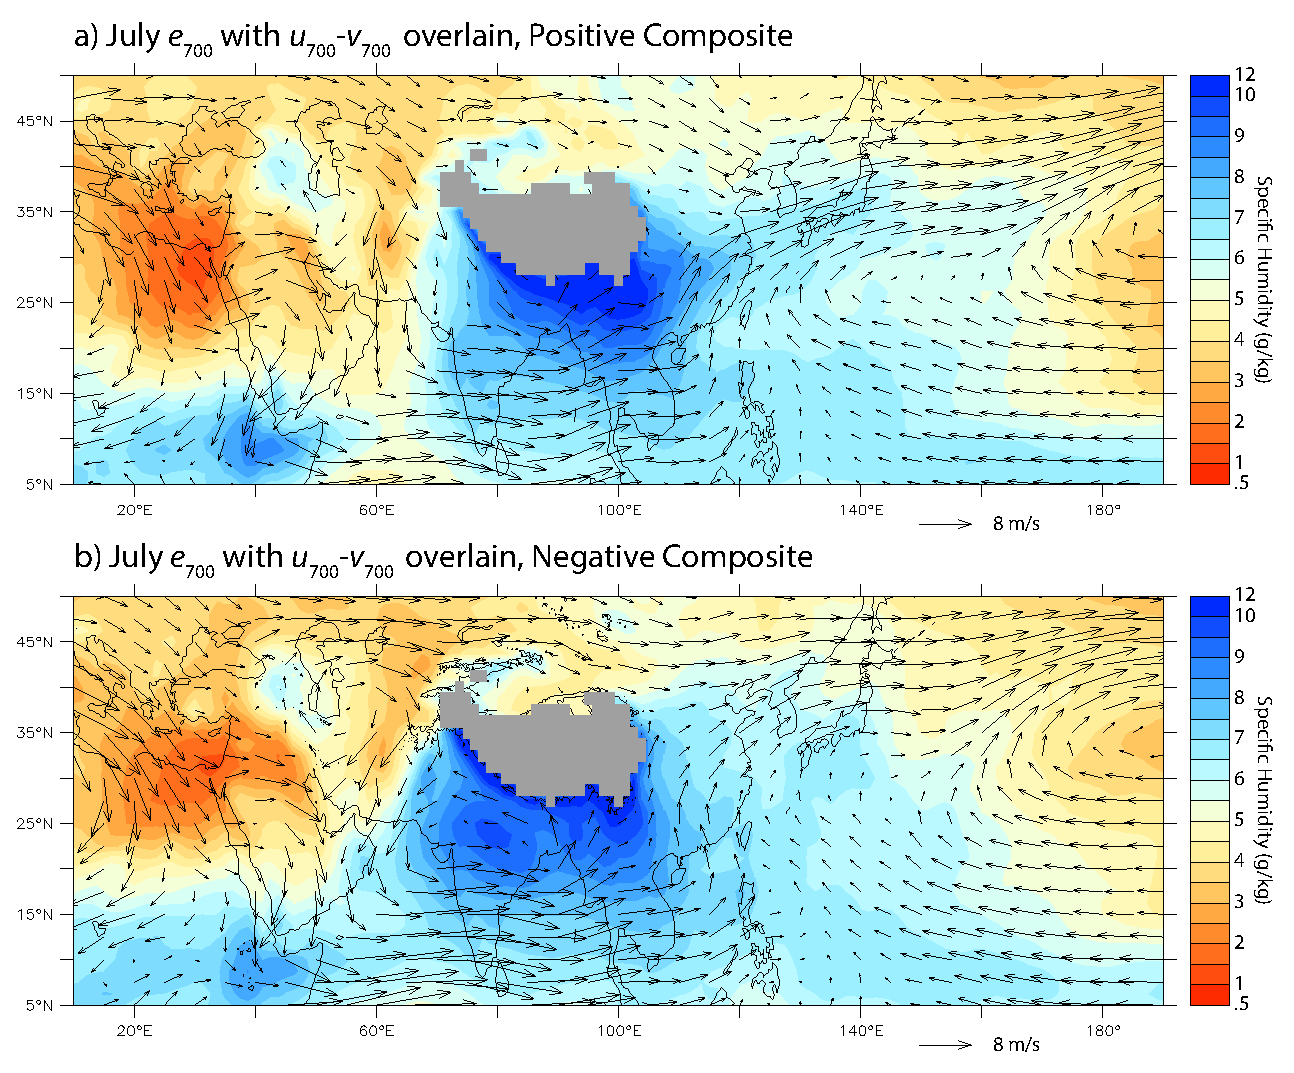
\includegraphics[width=36pc]{Figures/ch4/CGT_700}
\caption{JRA-55 700-mb specific humidity ($e_{700}$) with 700-mb level winds superimposed in a) a composite of positive All-Asia EOF1 years and b) for the negative All-Asia EOF1 composite. Since the scale height of water vapor is only about 3 km, we expect 700-mb winds to roughly match the direction of column-integrated moisture transport $qu-qv$.}
\label{fig:cgt_700}
\end{figure}

%% FIGURE 4.8 - Positive and negative composites of mid-tropospheric ascent and winds
\begin{figure}
\centering
\noindent\includegraphics[width=36pc]{Figures/ch4/CGT_500}
\caption{JRA-55 500-mb vertical pressure velocity $\omega_{500}$ (units of Pa/s, opposite sign from vertical velocity $w$) with 500-mb level winds superimposed for a) positive All-Asia EOF1 composite and b) negative All-Asia EOF1 composite.}
\label{fig:cgt_500}
\end{figure}

%% FIGURE 4.9 - All-Asia EOF1 variability looks locally like a jet shift.
\begin{figure}
\centering
\noindent\includegraphics[width=42pc]{Figures/ch4/CGT_u}
\caption{All-Asia EOF1 composite difference in JRA-55 200-mb level zonal wind (U200) for a) July and b) August. Regions of change between positive and negative All-Asia EOF1 composites that are significant at a 95\% confidence level are marked by stippling. The composite difference is marked by a southward shift of the East Asian Jet in positive All-Asia EOF1 years, and vice-versa in negative years. The overall pattern of change is significant at a 99\% confidence level. c) and d): JRA-55 fields of U200 in positive All-Asia EOF1 composite years for July and August respectively. e) and f): Same as Panels c and d, but for Negative All-Asia EOF1 composite years.}
\label{fig:cgt_u}
\end{figure}

%% FIGURE 4.10 Climatology of rainfall stages including rainfall, jet and most likely rainband configuration, and longitudinal averages.
\begin{figure}
\centering
\noindent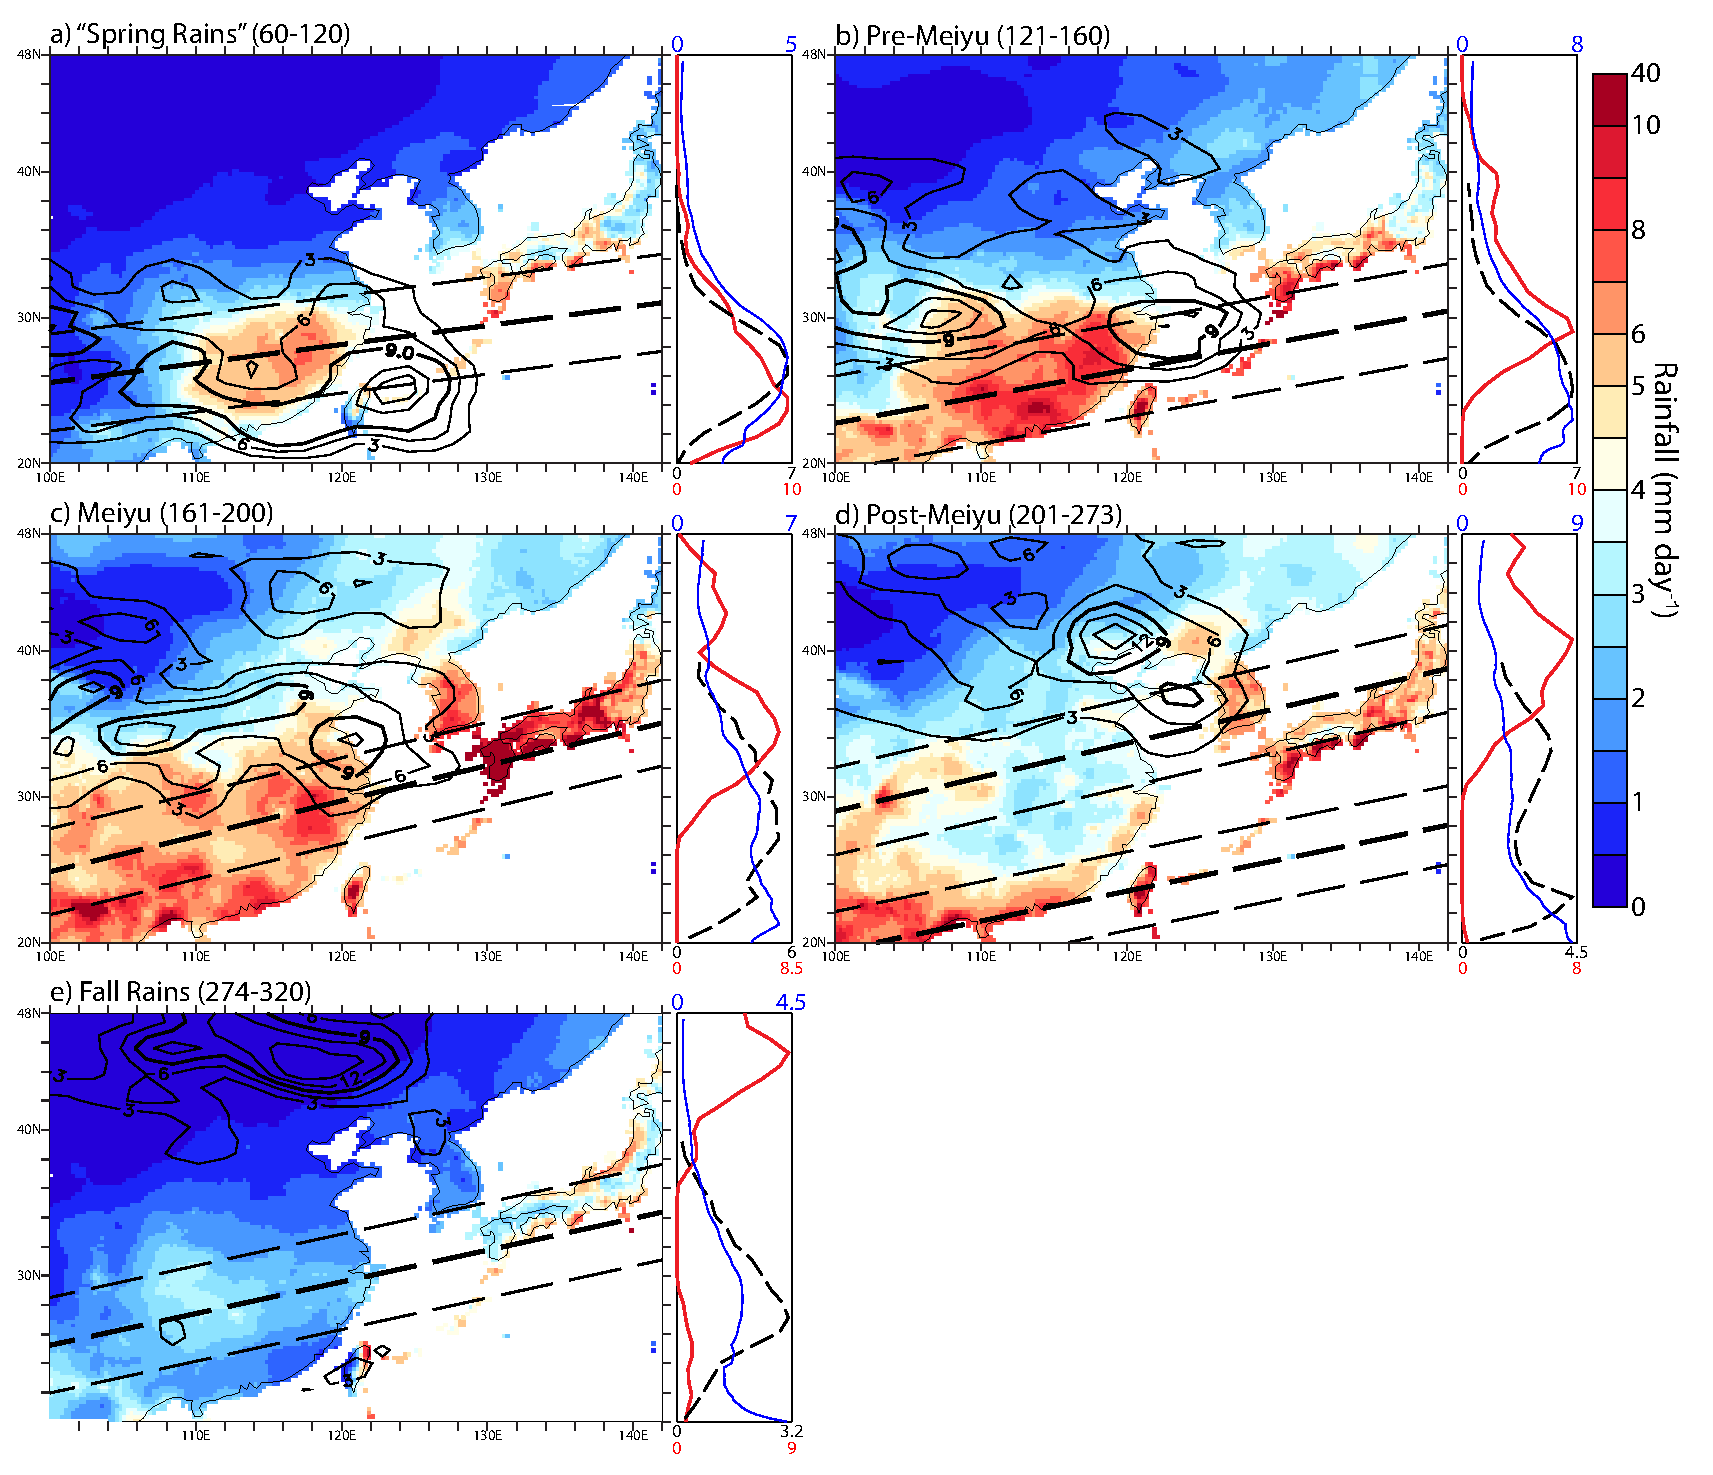
\includegraphics[width=36pc]{Figures/ch4/climo}
\caption{Climatology of East Asian rainfall stages showing rainfall (shading), jet kernel density (contours of probability density in units of $10^{-4}$) and most common rainband position during that stage. Sidebars shows, for each time period, the longitude average over 105-123$^{\circ}$E of rainfall (thin blue line, units of mm day$^{-1}$), jet kernel density (red line, units of $10^{-4}$) and rainband position (dashed black line, absolute probability in \%, 1-degree latitude smoothing). From the Pre-Meiyu to Post-Meiyu, a peak in preferred jet latitude consistently occurs 5 degrees north of a corresponding maximum in rainband frequency.}
\label{fig:climo}
\end{figure}

%% FIGURE 4.11 - Temporal autocorrelation of the jet used to demonstrate the choice of block size for averaging.
\begin{figure}[htbp]
\centering
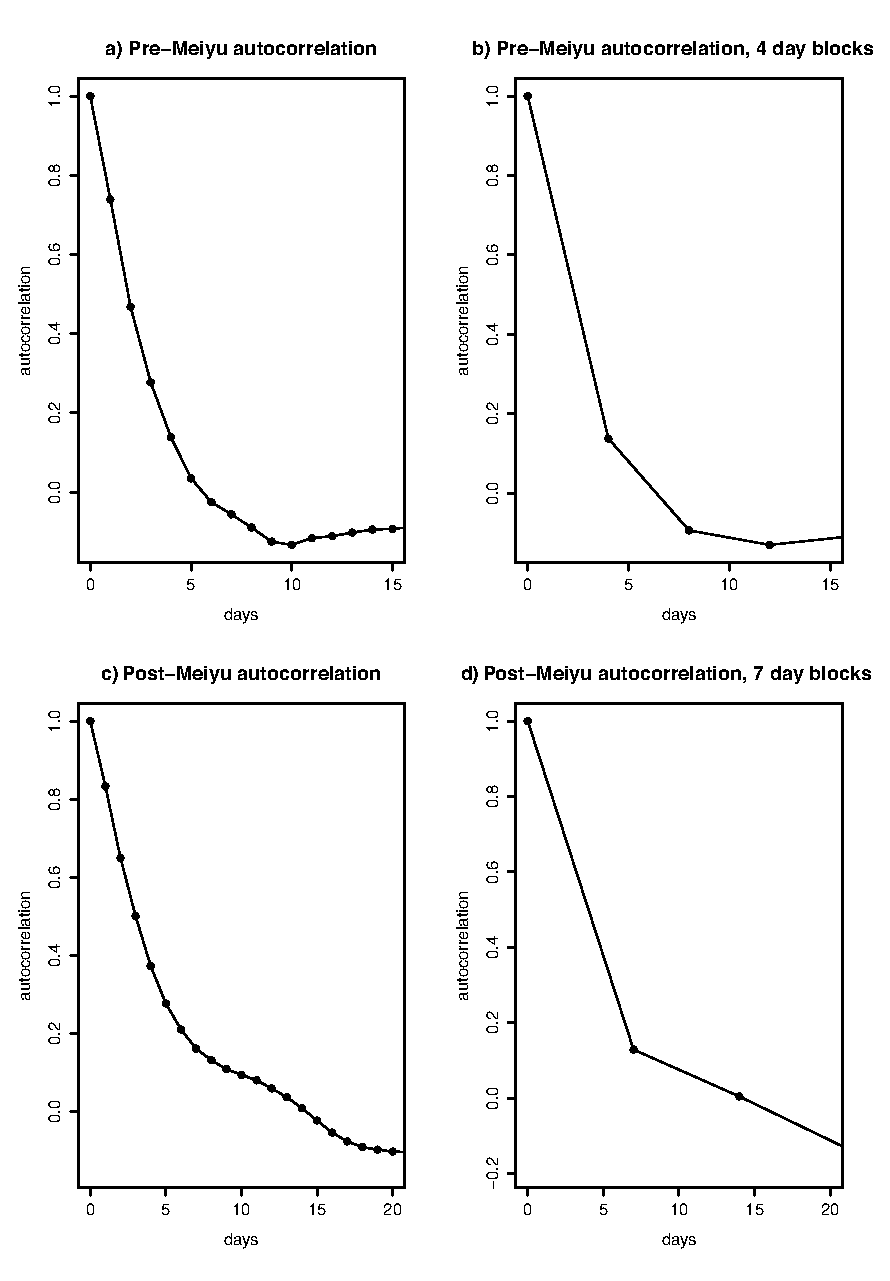
\includegraphics[width=24pc]{Figures/ch4/jet_autocorr}
\caption{The accumulation of the jet into blocks eliminates the autocorrelation from the daily mean latitude signal. During the Pre-Meiyu, mean daily jet latitude is further smoothed over 4 days (panels a and b); During the Post-Meiyu, we average over 7 days (panels c and d).}
\label{fig:jet_autocorr}
\end{figure}

%% FIGURE 4.12 - 2D spatial distribution of change showing a) full year b) Pre-Meiyu and c) Post-Meiyu
\begin{figure}
\centering
\noindent\includegraphics[width=36pc]{Figures/ch4/changes_2d_jet}
\caption{a) Whole year mean rainfall change for 1980-2001 versus 1958-1979, showing the South Flood-North Drought pattern; b) Rainfall changes during the Pre-Meiyu (days 121-160) with contours of jet density change overlain; c) Same as c, but for the Post-Meiyu (days 201-273). Statistical significance at 95\%/99\% level overlain with single/double hatches. Sidebars show, for each time period, the longitude average over 105-123$^{\circ}$E of changes in rainfall (thin blue line, units of mm day$^{-1}$), jet kernel density (red line, units of $10^{-4}$) and rainband position (dashed black line, absolute probability in \%, 1-degree latitude smoothing).}
\label{fig:changes_2d}
\end{figure}

%% FIGURE 4.13 - Changes in jet mean between 1951-1979 and 1980-2007 + scatter plots of jet and rainband monthly anomalies.
\begin{figure}[htbp]
\centering
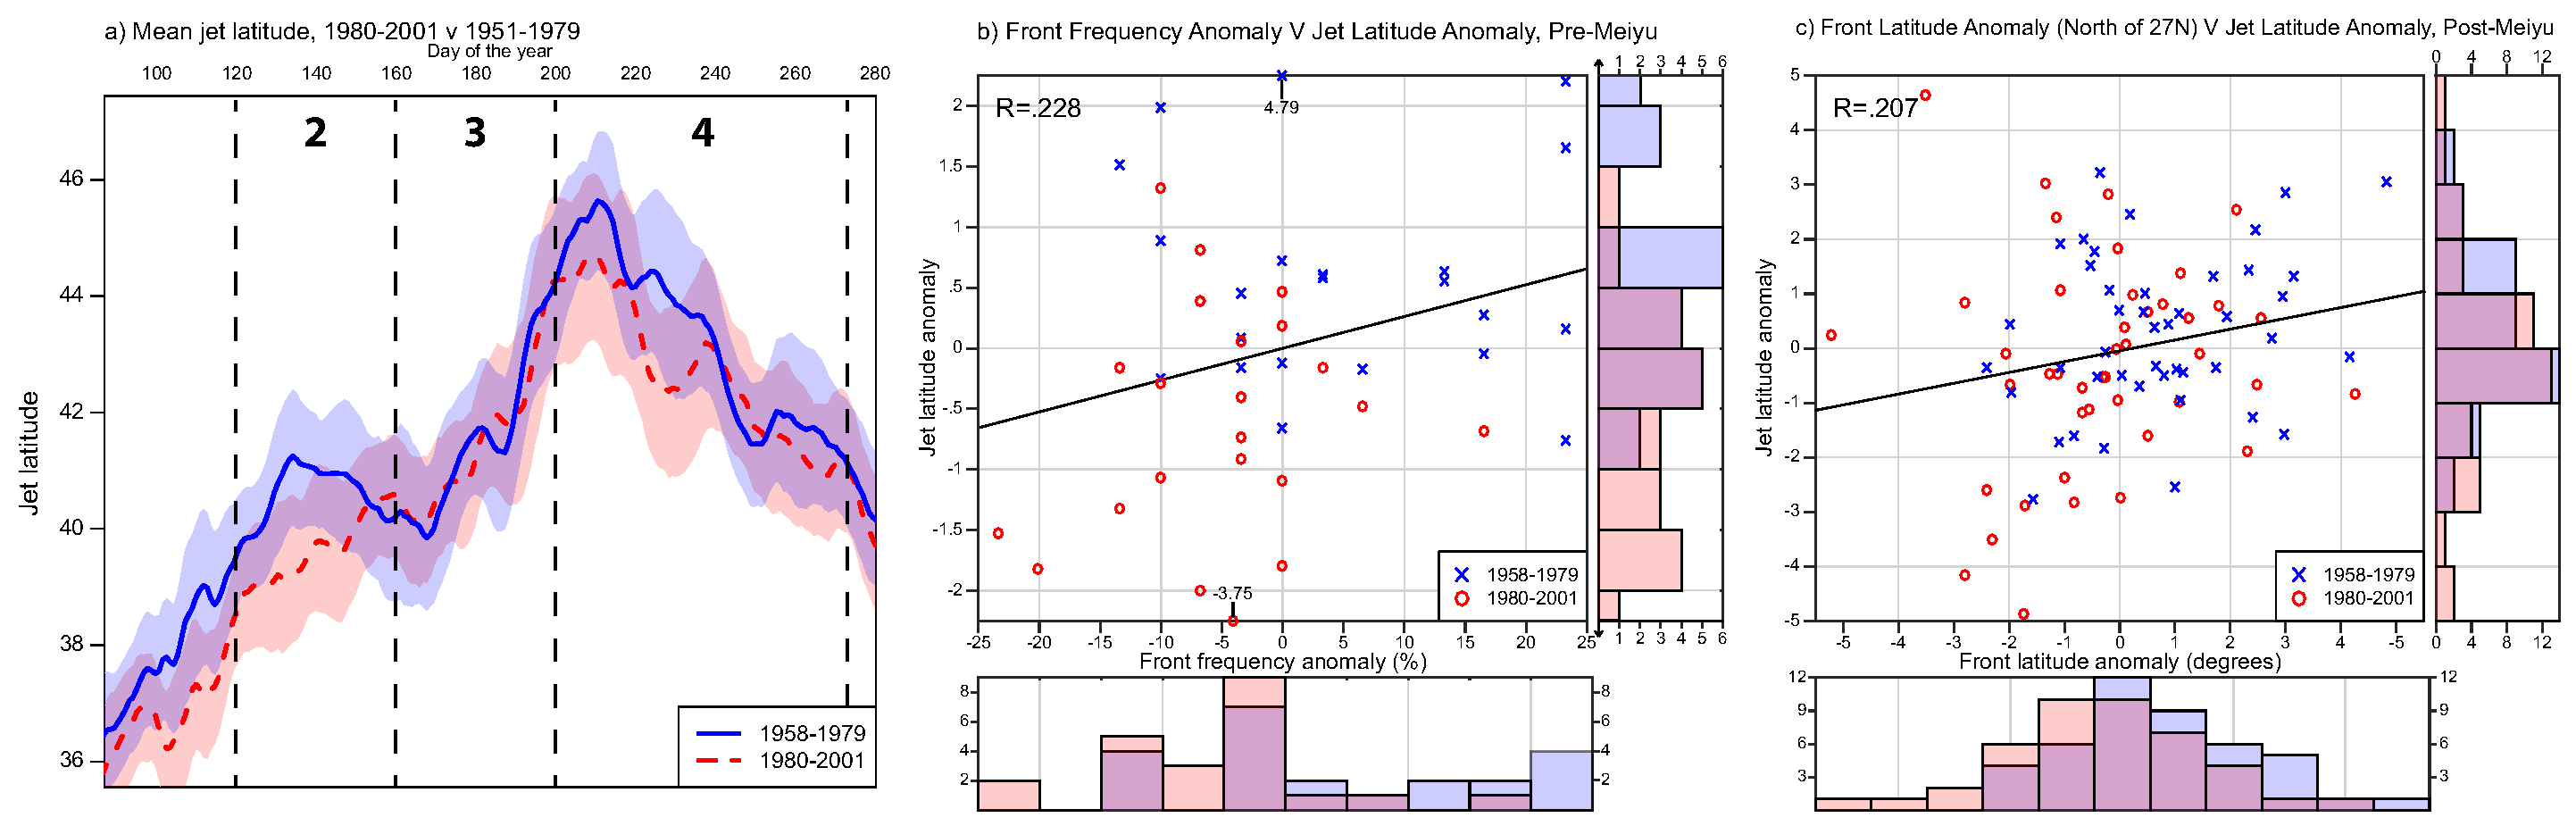
\includegraphics[width=42pc]{Figures/ch4/jet}
\caption{a) 7-day running mean latitude of the westerly jet in the region 90-130$^\circ$E for the years 1958-1979 (blue, solid) and 1980-2001 (red, dashed). Bootstrapped 95\% confidence intervals are shaded. Time periods: 2 - Pre-Meiyu; 3 - Meiyu; 4 - Post-Meiyu; b) Plot of monthly anomalies in rainband frequency versus monthly anomalies in jet latitude during days 121-150 (May) for 1958-1979 (blue X) versus 1980-2001 (red circle); c) Same as b), but showing 30-day anomalies of rainband latitudes during the Post-Meiyu (201-230 and 231-260, each set of 30 days treated as a separate point). Histograms of anomalies are also shown on the side of each figure.}
\label{fig:jet_seasonal}
\end{figure}


